%%%%%%%%%%%%%%%%%%%%%%%%%%%%%%%%%%
% Ch2 : Macro and micro balances %
%%%%%%%%%%%%%%%%%%%%%%%%%%%%%%%%%%$

\chapter{Macroscopic and microscopic balances}
\section{Conservation principles}
	The basic conservation principles in fluid mechanics are the conservation of \textbf{mass, energy and momentum.} These conservations are the basis of \textbf{continuity, Bernouilli and Navier-Stokes equations} and can be written in \textbf{integral} (finite volume of a mouving fluid) or \textbf{local} (balances in differential form) form. 
	
	\subsection{Macroscopic mass balance and continuity equation}
		\begin{wrapfigure}[4]{l}{4.5cm}
		\vspace{-5mm}
		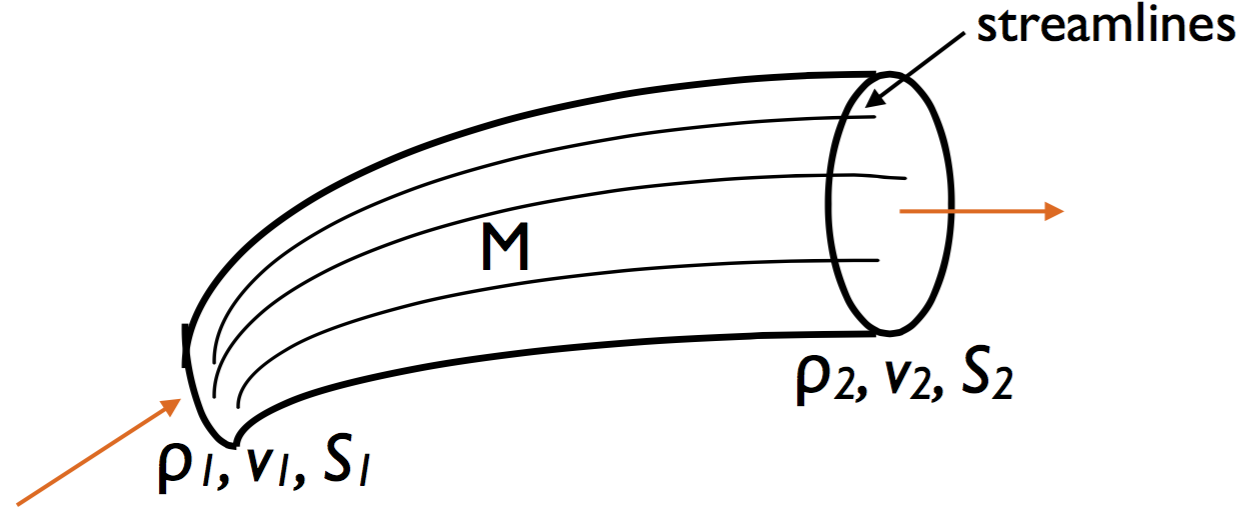
\includegraphics[scale=0.20]{ch2/1}
		\end{wrapfigure}
		In a steady\footnote{Continu, constant.} flow, the mass balance simply states that the mass entering is equal to the one leaving a volume. But we have to consider the variation of mass for transient\footnote{Transitoire.} problems. We define for that the  \textbf{mass flow rate} (débit) that gives the mass per time and is easy to measure. 
		\begin{equation}
			\dot{m} = \rho v S \qquad \qquad [\dot{m}] = \frac{[M]}{[T]}
		\end{equation}
		
		\subsubsection{General balance}
		Let's write what we explained, the mass variation is given by the mass entering at $S_1$ minus mass leaving at $S_2$		
		\begin{equation}
			\frac{dM}{dt} = \left(\rho \int _{S} v dS\right)_1 - \left(\rho \int _{S} v dS\right)_2
		\end{equation}
		To simplify, we introduce the \textbf{average velocity} $\bar{v} = \frac{1}{S}\int _S vdS$	giving the final expression
		\begin{equation}
			\frac{dM}{dt} = \left(\rho \bar{v} S\right)_1 - \left(\rho \bar{v} S\right)_2
		\end{equation}

		\subsubsection{Steady balance}
			When the fluid is steady, the velocity and the surface are constant in both 2 sections conducting to a constant mass
			\begin{equation}
				\dot{m} = \rho \bar{v}S = c
				\label{eq:2.4}
			\end{equation}

		\subsubsection{Streamlines}
			\begin{wrapfigure}[10]{r}{4.5cm}
			\vspace{-5mm}
			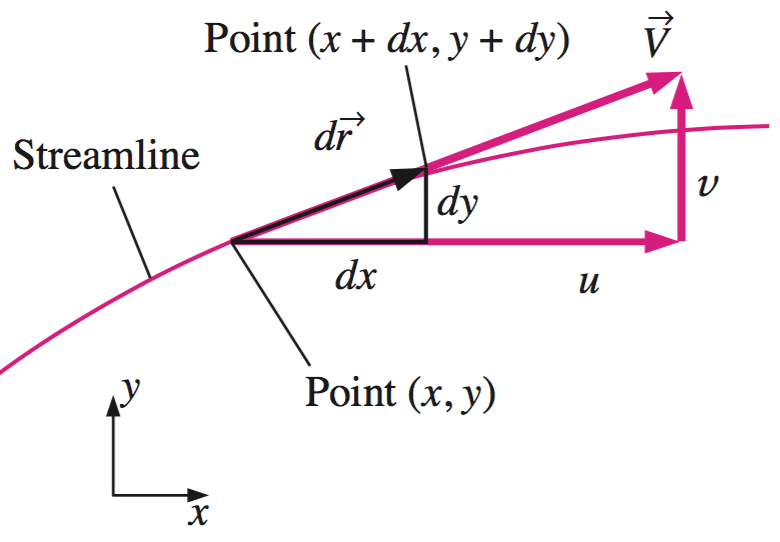
\includegraphics[scale=0.35]{ch2/2}
			\end{wrapfigure}
			Let's first define what's a streamline. It's a curve that is everywhere tangent to the instantaneous local velocity vector and so an indicator of the fluid direction. 
			Mathematically, if our velocity vector is 
			\begin{equation}
				\vec{V} = u\vec{i}+v\vec{j}+w\vec{k}
			\end{equation}
			we can take an infinetisimal arc length along a streamline 
			\begin{equation}
				d\vec{r} = dx\vec{i}+dy\vec{j}+dz\vec{k}
			\end{equation}
			Due to the 2 similar triangles, we have the relations \autoref{eq:2.7} that gives the 2D equation of a streamline.
			\begin{equation}
				\frac{dr}{V} = \frac{dx}{u} = \frac{dy}{v} = \frac{dz}{w} \qquad
				 \Rightarrow \qquad
				 \left(\frac{dy}{dx}\right)_{\mbox{along a streamline}} = \frac{v}{u}
				\label{eq:2.7}
			\end{equation}
			
	\subsection{Macroscopic momentum balance}
		Unlike the mass, momentum can be created and destroyed due to applied forces. The difference between the moementum entering in the control volume at $S_1$ and leaving at $S_2$ is equal to the sum of the forces applied to the fluid element. \\
		The momentum flow through a section per unit time is given by 
		\begin{equation}
			\dot{Q} = \dot{m}v = \rho \bar{v}^2 S
			\label{eq:2.8}
		\end{equation}
			and the forces acting on the fluid element (positive if exerted by the fluid) are :
			
		\begin{itemize}
				\item[•] \textbf{pressure} that is positive at the entry (the fluid push to enter) and negative at the exit (the fluid is pushed).
				\item[•] \textbf{forces on the walls} (normal and tangential). Negative because it's the reaction of the walls.
				\item[•] \textbf{Gravity and other volume forces}. Positive because the forces are due to the presence of a fluid volume. \\
		\end{itemize}

		It allows us to write the equation, considering that the surface is a vector of module equal to the scalar surface and of same direction of the normal to the surface. 
		\begin{equation}
			\sum F = p_1S_1 - p_2S_2 - F_w + F_g
			\label{eq:2.9}
		\end{equation}
		
		\subsubsection{Steady momentum balance}
			It's simply the use of equations \autoref{eq:2.8} and \autoref{eq:2.9}			
			\begin{equation}
				\dot{Q}_2 - \dot{Q}_1 = \sum F \qquad \Leftrightarrow \qquad \dot{m}_2v_2 - \dot{m}_1v_1 = p_1S_1 -p_2S_2 - F_w + F_g
			\end{equation}
			We can use equation \autoref{eq:2.4} and have a compact final relation 
			\begin{equation}
				\Delta ^2 _1 (\rho \bar{v}S + p) = -F_w+F_g
			\end{equation}
			
		\subsubsection{General momentum balance (transient)}
			To consider the case within the velocity is not constant into the 2 sections, we have to remind the mechanical relation for the resultant and do an infinitesimal deomposition in volume $V$	
			\begin{equation}						
			\begin{aligned}
				\frac{dR}{dt} = \sum F \qquad \Leftrightarrow \qquad \frac{d}{dt}\int _V \rho v dV &= (\rho \bar{v}^2 +p)_1S_1 - (\rho \bar{v}^2 +p)_2S_2 - F_w + F_g \\
				&= \Delta ^2 _1 (\rho \bar{v}^2  +p)S-F_w+F_g
			\end{aligned}
			\end{equation}
			You can find an example of exercice on slide 8 and 9 where we study the forces on an elbow\footnote{Coude}. Keep in mind that we often \textbf{consider a steady-state flow} to simplify $d/dt = 0$.
			
		\subsection{Local form of the conservation principles}
			\subsubsection{Macroscopic balances}
				They are used to have a general view an a volume, when we are interested in the \textbf{overall features}\footnote{Caractéristiques générales}.
			\subsubsection{Microscopic balances}
				They consist on differantial and local equations and are valid on every point of the fluid to give the velocity, density or pressure. 

\section{Continuity equation}
	\begin{wrapfigure}[7]{l}{3cm}
		\vspace{-5mm}
		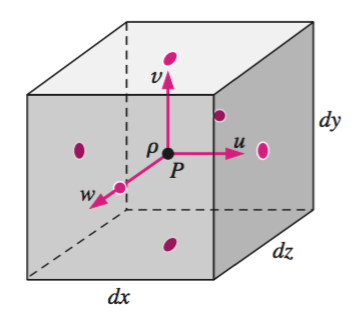
\includegraphics[scale=0.5]{ch2/3}
		\end{wrapfigure}
			The continuity equation caracterise the net rate of change of mass in a control volume. We start from the fact that this rate is equal to the net rate at wich mass flows through the volume. \\
			
			The variation of mass in function of time in an infinitesimal volume is given by 
			\begin{equation}
				\partial M = \frac{\partial \rho}{\partial t} \partial x \partial y \partial z
			\end{equation}
			If we do the difference between the enter and the exit of the flow in the volume following axis x, we have $(\rho v S)$
			\begin{equation}
				\rho u \partial y \partial z - \left( \rho u + \frac{\partial (\rho u)}{\partial x}\partial x \right) \partial y \partial z
				= - \frac{\partial (\rho u)}{\partial x}\partial x \partial y \partial z
			\end{equation}
			and using the same way for the other axis
			\begin{equation}
				- \frac{\partial (\rho v)}{\partial y}\partial x \partial y \partial z
				 \qquad and \qquad 
				- \frac{\partial (\rho w)}{\partial z}\partial x \partial y \partial z
			\end{equation}
			We take care of the contributions in all direction and simplify the infinitesimal volume in each term
			\begin{equation}
				\frac{\partial \rho}{\partial t} + \frac{\partial (\rho u)}{\partial x} + \frac{\partial (\rho v)}{\partial y} + \frac{\partial (\rho w)}{\partial z} = 0 
				\qquad \Rightarrow \qquad
				\frac{\partial \rho}{\partial t} + \nabla (\rho v) = 0
			\end{equation}
			Where the final $v$ is global and not specific to an axis. Let's remind that the material derivative is defined as $\frac{D\rho}{Dt} = \frac{\partial \rho}{\partial t} + v \nabla \rho$, we have
			\begin{equation}
				\frac{D\rho}{Dt} + \rho \nabla v = 0
			\end{equation}
			
\section{Momentum equation}
\subsection{Cauchy equation}
	To solve this rapidly we use the Langrangian approach. We suppose that the control volume is moving with the fluid and contain a fixed mass. The momentum rate of change is is equal to the net force acting on the control volume (volumetric and superficial)
	\begin{equation}
		\frac{D}{Dt} \int _{V_m(t)} \rho v \, dV = \int _{V_m(t)} \rho g \, dV + \int _{S_m(t)} f \, dS
		\label{eq:2.18}
	\end{equation}
	$f$ is a function of the position $r$ on the surface defined by the unit vector $n$ perpendicular to the surface and pointing outward. $f$ can be expressed as the scalar product between the tensor $T$ and normal $n$
	\begin{equation}
		f(n,r) = nT(r)
		\label{eq:2.19}
	\end{equation}
	
		\begin{wrapfigure}[10]{r}{5cm}
		\vspace{-5mm}
		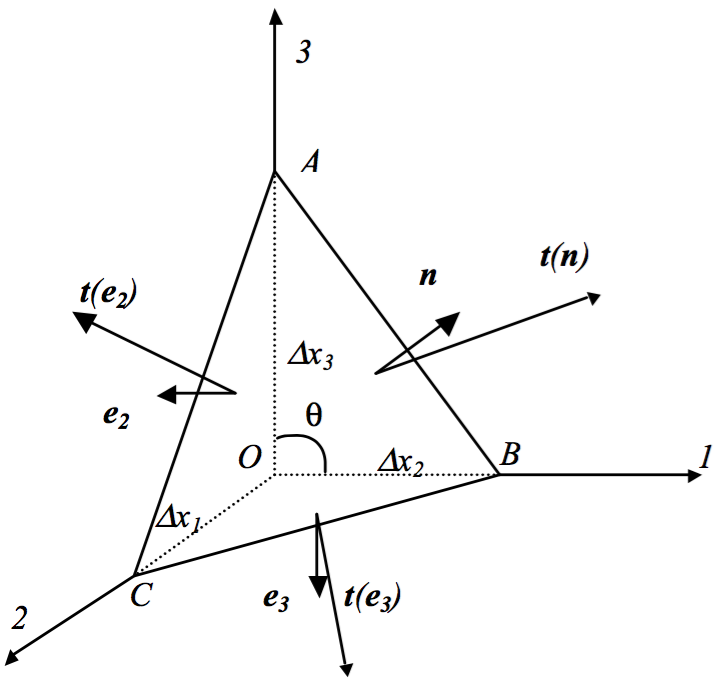
\includegraphics[scale=0.4]{ch2/4}
		\end{wrapfigure}
		Let's consider a tetrahedron on the axis $x_1,x_2,x_3$ and the forces exerted by the surrounding fluid. The force balance can be expressed 
		\begin{equation}
		\begin{aligned}
			f(n) S_{ABC} &= f(e_1) S_{AOB} + f(e_2) S_{AOC} + f(e_3) S_{BOC} \\
			&= f(e_1) S_{ABC} n e_1 + f(e_2) S_{ABC} n e_2 + f(e_3) S_{ABC} n e_3
			\end{aligned}
		\end{equation}
		if we do a factorisation and we define the tensor $T$ as
		\begin{equation}
			T = e_1f(e_1)+e_2f(e_2)+e_3f(e_3)
		\end{equation}
		we find the equation \autoref{eq:2.19}. We can so write the equation \autoref{eq:2.18} with this expression and use the \textbf{divergence theorem}
		\begin{equation}
			\int _S nT \, dS = \int _V \nabla T \, dV 
		\end{equation}
		we obtain the equation 
		\begin{equation}
			\int _V \left[ \frac{\partial (\rho v)}{\partial t} + \nabla (\rho vv) - \nabla T - \rho g \right] dV = 0
		\end{equation}
		Considering that it must be valid for any and every point of the volume, we get the \textbf{Cauchy equation}\footnote{We can get $\rho$ out of the material derivative because we consider a constant $\rho$}
		\begin{equation}
			\rho \frac{Dv}{Dt} = \nabla T + \rho g
			\label{eq:cauchy}
		\end{equation}

	\subsection{Constitutive equations}
		\subsubsection{Static conditions}
			Imagine that we have a static fluid. The only force $f$ will be due to the pressure $p$ 
			\begin{equation}
				f = -pn \Leftrightarrow T = -pI = 
				\left(
				\begin{array}{ccc}
				-p & 0 & 0 \\ 
				0 & -p & 0 \\ 
				0 & 0 & -p
				\end{array} 
				\right)
			\end{equation}
			In that case, the use of equation \autoref{eq:cauchy} give us the information
			\begin{equation}
				\rho g = \nabla p
			\end{equation}
			
		\subsubsection{Dynamic conditions}
			Let's now take care of the viscosity effects on a Newtonian fluid. In that case we have to add to the pressure the forces function of the velocity gradient 
			\begin{equation}
				T = -pI + f(\nabla v)
			\end{equation}
			where $(\nabla v)$ has a symetrical (pure deformations) and an antisymetrical (pure rotation) part given by
			\begin{equation}
				S = \frac{1}{2}(\nabla v + \nabla v ^T) \qquad and \qquad A = \frac{1}{2}(\nabla v - \nabla v ^T)
			\end{equation}
		
		\subsubsection{Final form of the stress tensor}
		Given the upper discussion, the final expression is 
		\begin{equation}
			T = \left[ -p + \lambda (\nabla v) \right]I + 2\mu S	
		\end{equation}		 
		where $S$ is the symetric part of the gradient. Let's precise that for \textbf{incompressible flows}, we have
		\begin{equation}
			T = -pI + 2\mu S
			\label{eq:incompressible}
		\end{equation}
		
		\subsubsection{Navier-Stokes equation}
		\theor{\textsc{Navier-Stokes equation}\\
		For incompressible, Newtonian and isothermal flows 
		\begin{equation}
			\rho \frac{Dv}{Dt} = \rho \left[ \frac{\partial v}{\partial t} + v\nabla v  \right] = - \nabla p + \mu \nabla^2 v + \rho g
			\label{eq:navier}
		\end{equation} }
		\ \\ Where we used the Cauchy equation \autoref{eq:cauchy} and equation \autoref{eq:incompressible} for $T$. 
		
\section{Bernouilli equation}
	\subsection{Without friction effects and energy transfer}
	To access the Bernouilli equation, let's take the Navier-Stokes equation \autoref{eq:navier} and disregard the viscous term (with $\mu$). The scalar multiplication of that equation provides the \textbf{kinetic energy balance}
	\begin{equation}
		\rho v \frac{Dv}{Dt} = \rho \frac{D}{Dt} \frac{v^2}{2} = -v\nabla (p + \rho \Phi) 
		\qquad with \qquad 
		\Phi = g
		\left(
		\begin{array}{c}
		0 \\
		0 \\
		z
		\end{array}
		\right)
	\end{equation}
	For incompressible and steady fluids, $\frac{d\rho}{dt} = 0 = \frac{dp}{dt}$, so 
	\begin{equation}
		\frac{D}{Dt}\left( \rho \frac{v^2}{2} + p + \rho g z \right)	 = 0 
	\end{equation}	 
		leading us to the Bernouilli equation after integration. \\
		
		\theor{\textsc{Bernouilli equation}\\
		The sum of the kinetic, potential and flow energies of a fluid particle is \textbf{constant} along a streamline during \textbf{steady} flow when the \textbf{compressibility} and \textbf{frictional effects} are negligible. 
		\begin{equation}
			\rho \frac{v^2}{2} + p + \rho g z = c = p_{tot}
		\end{equation}
		\begin{itemize}
			\item[•] $\frac{v^2}{2}$ is the \textbf{dynamic pressure} : pressure rise when the fluid in motion is brought to a stop isentropically. 
			\item[•] $p$ is the static pressure : thermodynamic pressure of the fluid.
			\item[•] $\rho g z$ is the \textbf{hydrostatic pressure} : for the elevation effects.
		\end{itemize} }
		\ \\ Finally, we can say that the sum of these 3 type of pressure is the \textbf{total pressure} and that it's constant along a srteamline. 

		\subsubsection{Limitations of the Bernouilli equation}
			To use Bernouilli equation we have to make some hypothesis : 
			\begin{itemize}
				\item[•] \textbf{Steady flow} : cannot be used for transients (start-up and shut-down) flow or with changes in flow conditions. 
				\item[•] \textbf{Frictionless flow} : cannot be used when there are components disturbing the flow.
				\item[•] \textbf{No shaft work} : cannot use in presence of pump, turbine, etc (destroy the streamline structure).
				\item[•] \textbf{Incompressible flow} : cannot be used when the density changes. Liquids and gases (Mach numbers $<0.3$) are ok.
				\item[•] \textbf{No heat transfer} : the increase of temperature influe on the density.
				\item[•] \textbf{Along a streamline} : the constant $c$ is the same for all streamlines if the flow is irrotational.
			\end{itemize}				
			Many applications exists like the the Pitot tube, the cavitation or the discharge of a fluid from a tank. 
			
			\subsection{With friction effects and energy transfer}
				We have to generalize the Bernouilli equation. To take care of the friction forces that dissipate the mechanical energy into heat, we introduce a \textbf{pressure drop} $\Delta P_{tot}$ for \textbf{incompressible fluids}. Friction is an \textbf{irreversible process} and this forces are always positive (for potential flow = 0). \\
				When pumps and turbines are used, we introduce an \textbf{energy transfer by work} $w_p$ and $w_t$. The contributions for pumps are positive whereas they are negative for turbines 
				\begin{equation}
					\rho \frac{v_1^2}{2} + p_1 + \rho gz_1 + w_p -w_t - \Delta P_{tot} = c
				\end{equation}
				
\section{Distributed pressure drops}
	\begin{wrapfigure}[3]{l}{5cm}
	\vspace{-5mm}
	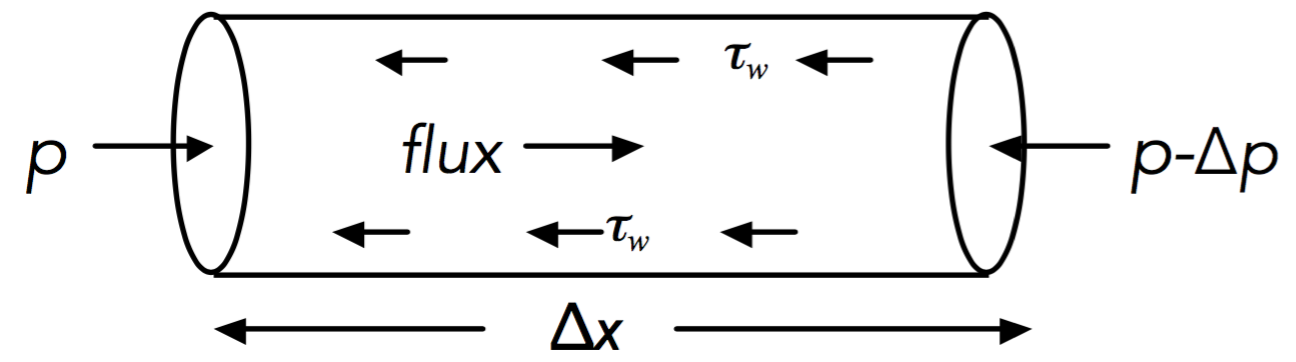
\includegraphics[scale=0.2]{ch2/5}
	\end{wrapfigure}
	We want to determine the pressure drops for internal flows. Let's begin with the energy balance 
	\begin{equation}
			\rho \frac{v_2^1}{2} + p_1 + \rho gz_1 + w_p = \rho \frac{v_2^2}{2} + p_2 + \rho gz_2+w_t + \Delta P_{tot}
	\end{equation}
	After simplifying the relation, we find that 
	\begin{equation}
		\Delta p = \Delta P_{tot} 
		\label{eq:2.37}
	\end{equation}
	Let's now do the force balance consisting on the pressure force at the entry, the exit and the shear stress whithin the volume
	\begin{equation}
		\sum F = \pi R^2 p - \pi R^2 (p-\Delta p) - (2\pi R \Delta x)\tau _{w} = 0 
	\end{equation}
	After simplifying the terms and isolating the ratio, we can use the relation \autoref{eq:2.37}
	\begin{equation}
		\frac{\Delta p}{\Delta x} = \frac{2\tau _w}{R} = \frac{4 \tau _w}{D} \qquad \Rightarrow \qquad \Delta P_{tot} = \frac{2\tau _w}{R} = \frac{4 \tau _w}{D} L
	\end{equation}
	Let's finally introduce the \textbf{Moody coefficient} $\lambda$ and the \textbf{Fanning coefficient} $\mathbf{f}$ to obtain the final expression 
	\begin{equation}
		\lambda = 4f = 4\frac{\tau _w}{\frac{\rho v^2}{2}} \qquad \Rightarrow  \qquad \Delta P_{tot} = \lambda\frac{L}{D}\frac{\rho v^2}{2}
	\end{equation}

\section{Newtonian flow in a pipe}
	\subsection{Case of a laminar regime (Re < 2100)}
		\begin{wrapfigure}[3]{r}{4.5cm}
		\vspace{-15mm}
		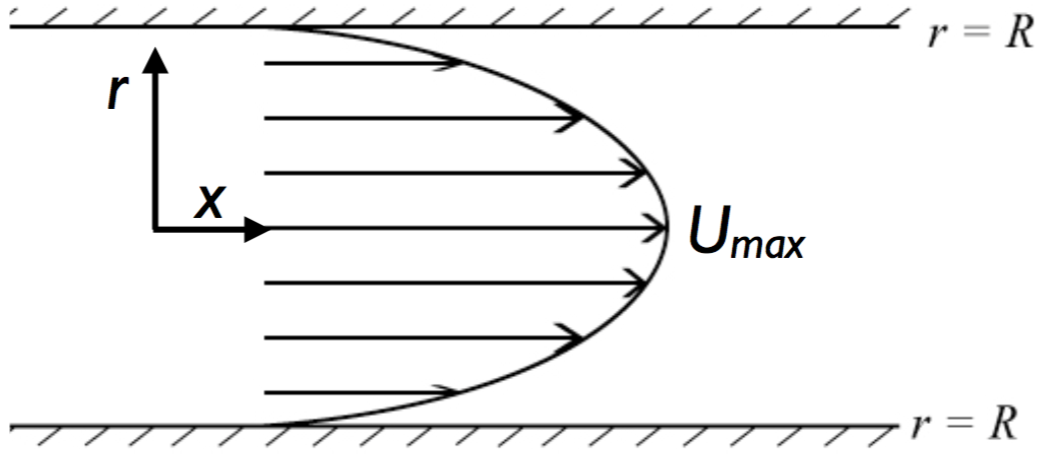
\includegraphics[scale=0.25]{ch2/6}
		\end{wrapfigure}
		Let's take the Nvier-Stokes equation \autoref{eq:navier} and suppose that there is no gravity effect on the fluid and that the flow is \textbf{steady}. 
		\begin{equation}
			\cancel{\rho \frac{Dv}{Dt}} = -\nabla p + \mu \nabla ^2 v + \cancel{\rho g} 
			\qquad \Rightarrow \qquad 
			0 = -\underbrace{\frac{\partial p}{\partial x}}_{f(x)} + \frac{\mu }{r} \frac{\partial}{\partial r} \underbrace{\left( r\frac{\partial u}{\partial r}\right)}_{f(r)}
		\end{equation}

		The pressure pressure drop per unit lenght $\frac{\Delta p}{L}$ must be constant because of the steady regime and the sections are equivalent
		\begin{equation}
			\frac{1}{\mu}\frac{\partial p}{\partial x} = \frac{1}{r} \frac{\partial}{\partial r} \left( r\frac{\partial u}{\partial r} \right) = c = - \frac{\Delta p}{\mu L}
		\end{equation}
		The non-slip conditions on the walls ($r=R$) impose that $U = 0$ and the maximum velocity at $r=0$ impose that $\frac{du}{dr} = 0$. The integration part per part gives
		\begin{equation}
			d \left( r\frac{\partial u}{\partial r} \right) = - \frac{\Delta p}{\mu L} r\, dr 
			\qquad \Rightarrow 
			\frac{\partial u}{\partial r} = -\frac{\Delta p}{\mu L} \frac{r}{2} + \frac{C_1}{r} 
			\qquad \Rightarrow 
			u(r) = -\frac{\Delta p}{\mu L} \frac{r^2}{4} + C_1 \ln r + C_2 
		\end{equation}
		The upper conditions give the value of constants $C_1 = 0$ and $C_2 = \frac{\Delta p}{\mu L}\frac{R^2}{4}$. \\
		
		It enable us to calcul the :
		\begin{itemize}
			\item[•] velocity profile
			\begin{equation}
				U = \frac{\Delta p}{16\mu L}D^2 \left(1-\left(\frac{r}{R}\right)^2 \right)
			\end{equation}
			
			\item[•] Maximum velocity 
			\begin{equation}
				U_{max} = \frac{\Delta p}{16 \mu L }D^2
			\end{equation}
			
			\item[•] Volumetric flow rate
			\begin{equation}
				\dot{V} = \int _0 ^r 2\pi r u(r) \, dr = \frac{\pi}{128 \mu} \frac{\Delta p D^4}{L}
			\end{equation}
			
			\item[•] Mean speed (vitesse moyenne)
			\begin{equation}
				\frac{\dot{V}}{S} = \frac{\pi}{128 \mu} \frac{\Delta p D^4}{L} \frac{4}{\pi D^2} = \frac{U_max}{2}
			\end{equation}
			
			\item[•] Wall shear stress
			\begin{equation}
				\tau _{max} = -\mu |\frac{du}{dr}| _{r=R} = \frac{4 \mu \bar{U}}{R}
			\end{equation}
			
			\item[•] Friction coefficient
			\begin{equation}
				f = \frac{\lambda}{4} = \frac{4 \mu \bar{U}}{\frac{1}{2}\rho \bar{U}^2 R} = \frac{8 \mu \bar{U}}{\frac{1}{2}\rho \bar{U}^2 D} = \frac{16}{Re}
			\end{equation}
		\end{itemize}
		
	\subsection{Case of a turbulent regime (Re > 3500)}
		We have to consider two case in that case. When the walls are smooth\footnote{Lisse}, the Moody coefficient is given by 
		\begin{equation}
			\lambda = \frac{0.316}{Re_D^{0.25}}
		\end{equation}
		When the walls are rough\footnote{Rugueux}, we have the \textbf{Nikuradse equation} and the \textbf{Colebrook equation}
		\begin{equation}
			\frac{1}{\sqrt{\lambda}} = 1.14 - 0.868 \, \ln \bar{\Lambda}
			\qquad and \qquad
			\frac{1}{\sqrt{\lambda}} = 1.14 - 0.868 \, \ln \left(\bar{\Lambda}+\frac{9.34}{Re\sqrt{\lambda}} \right)
		\end{equation}
\begin{center}
		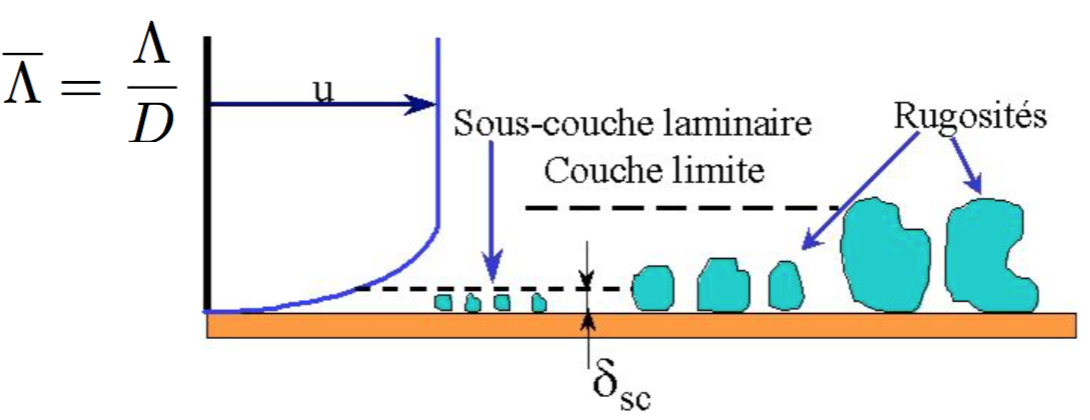
\includegraphics[scale=0.4]{ch2/7}
\end{center}
I REALLY DON'T HAVE UNDERSTOOD ! PLEASE COMPLETE WITH YOUR NOTES.

\section{Concentrated pressure drops}
	They are caused by inlets and outlets, curves, change in the cross section, offtakes\footnote{Prélèvements}, ... \\
	They are modelled simirarly to the distributed pressure drops with the \textbf{lack-of-knowledge coefficient} $K$ that differs by geometries and configurations
	\begin{equation}
		\Delta P_{tot,c} = \sum _j K_j \frac{\rho U_j^2}{2}
	\end{equation}
	
	\begin{wrapfigure}[3]{l}{8cm}
	\vspace{-5mm}
	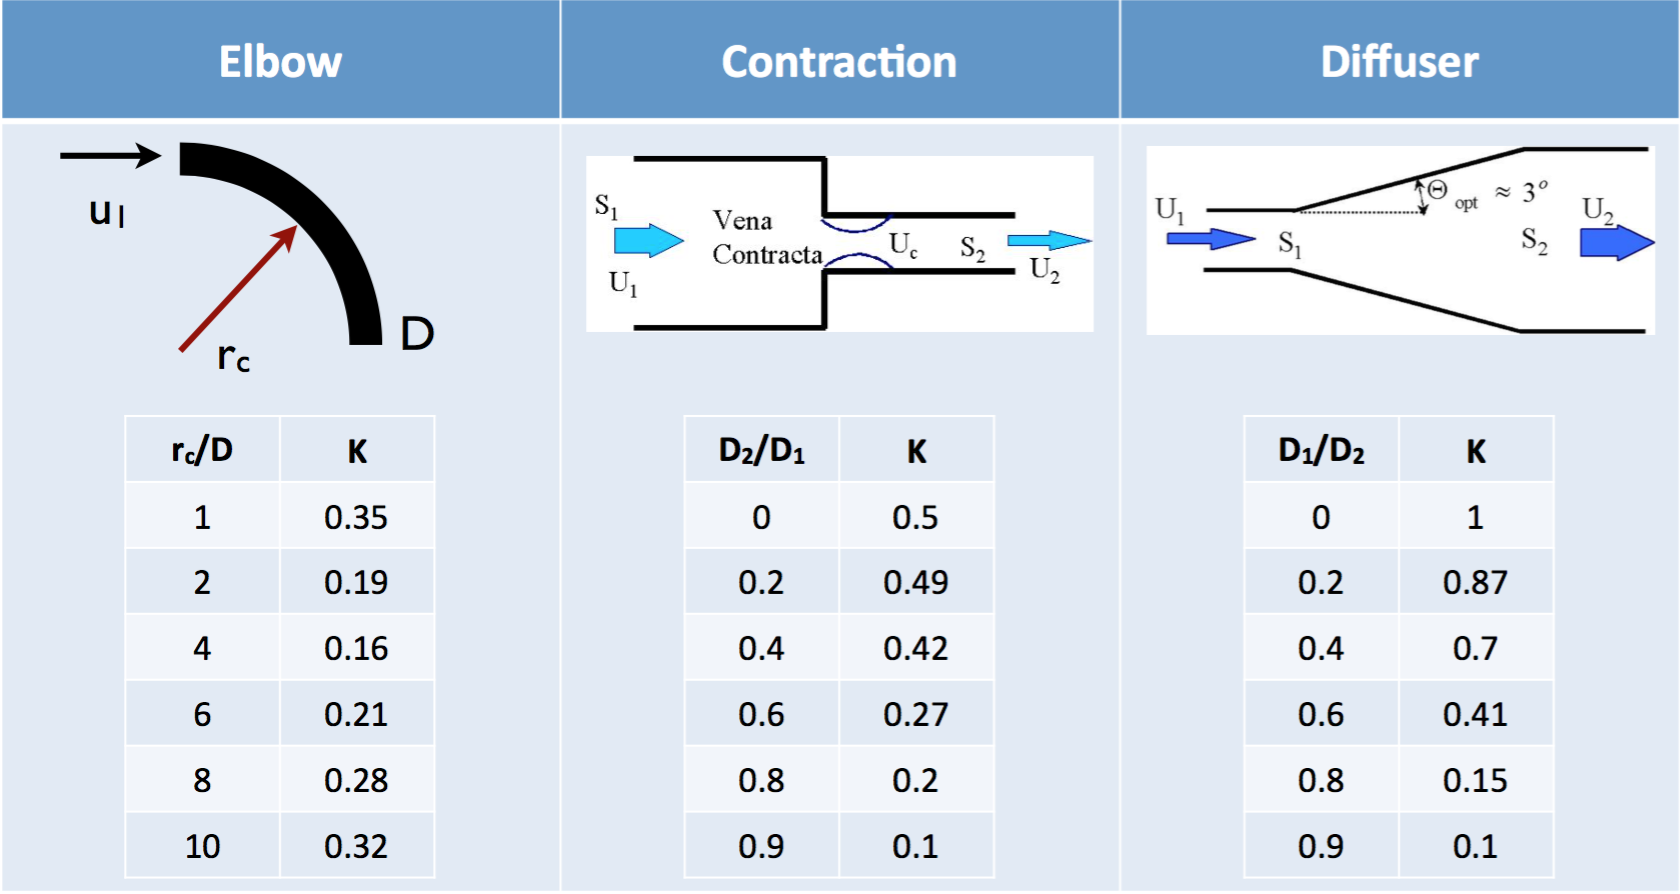
\includegraphics[scale=0.25]{ch2/8}
	\end{wrapfigure}
	Here you can find some values for different situations. \\\\\\\\\\\\\\
	We can now establish the total pressure drops expression 
	\begin{equation}
		\Delta P_{tot} = \Delta P_{tot,d} + \Delta P_{tot,c} = \sum _i \lambda _i \frac{L_i}{D_i}\frac{\rho U_i^2}{2} + \sum _j K_j \frac{\rho U_j^2}{2}
	\end{equation}	 
	
	\subsubsection{Hydraulic diameter}
		To evaluate the Reynolds number we introduce the hydraulic diameter defined by 
		\begin{equation}
			D_h = 4\frac{S}{P}
		\end{equation}
		Where $S$ is the surface, $P$ the perimeter and the value 4 is introduced to retrieve the normal diameter for a circular section. Let's calcul this diameter.
		\begin{center}
		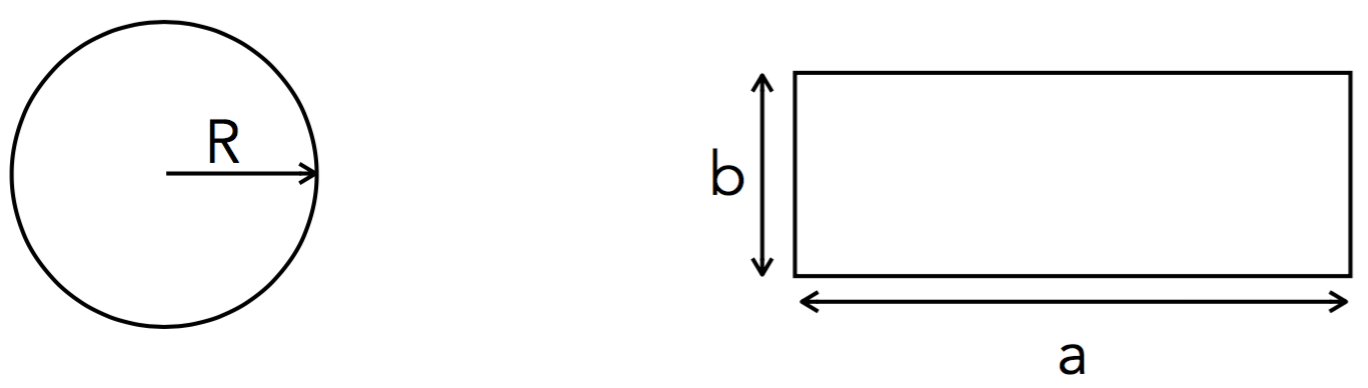
\includegraphics[scale=0.4]{ch2/9}
		\end{center}
		\begin{equation}
			D_h = 4\frac{\pi R^2}{2\pi R} = D \qquad\qquad and \qquad\qquad D_h = 4 \frac{ab}{2a+2b} \approx 2b
		\end{equation}
		Finally, we can find the Reynolds number by
		\begin{equation}
			Re_h = \frac{D_hU}{\nu}
		\end{equation}